\section{Test Description and Success Criteria}
This test is located at {\tt SimCode/sensors/imu\_sensor/\_UnitTest/test\_imu\_sensor.py}. In order to get good coverage of all the aspects of the module, the test is broken up into several parts: \par

\subsection{Primary Test Method}
In order to thoroughly test arbitrary outputs from the IMU, The equations of motion for the sensor were formulated as functions of the center of mass of the spacecraft as opposed to the equations seen in the model description which were formulated about the body frame. The truth values for the following test are set up in the following way:
\begin{equation}
{\bm{r}}_{S/N} = {\bm{r}}_{C/N} + {\bm{r}}_{S/C}
\end{equation}
\begin{equation}
\dot{{\bm{r}}}_{S/N} = \dot{{\bm{r}}}_{C/N} + {\bm{r}}'_{S/C} + \bm{\omega}_{B/N} \times {\bm{r}}_{S/C}
\label{eq:firstder}
\end{equation}
Knowing that:
\begin{equation}
{\bm{r}}'_{S/C} = - \bm{c}'
\end{equation}
Eq. \ref{eq:firstder} becomes:
\begin{equation}
	\dot{{\bm{r}}}_{S/N} = \dot{{\bm{r}}}_{C/N} - \bm{c}' + \bm{\omega}_{B/N} \times {\bm{r}}_{S/C}
	\label{eq:rdot}
\end{equation}
So, again substituting in the center of mass velocity in the $\cal{B}$ frame,
\begin{equation}
\ddot{{\bm{r}}}_{S/N} = \ddot{{\bm{r}}}_{C/N} - \bm{c}'' - 2\bm{\omega}_{B/N} \times \bm{c}'  + \dot{\bm{\omega}}_{B/N} \times {\bm{r}}_{S/C} + \bm{\omega}_{B/N} \times \bm{\omega}_{B/N} \times {\bm{r}}_{S/C}
\label{eq:SN}
\end{equation}
$ \bm{c}''$ and $ \bm{c}'$ can be solved for in terms of $\ddot{\bm{c}}$ and $\dot{\bm{c}}$ using the transport theorem:
\begin{equation}
\bm{c}'   = \dot{\bm{c}} - \bm{\omega}_{B/N} \times \bm{c}
\end{equation}
\begin{equation}
\bm{c}''  = \ddot{\bm{c}}  - 2\bm{\omega}_{B/N} \times \bm{c}' - \dot{\bm{\omega}}_{B/N} \times \bm{c}  -\bm{\omega}_{B/N} \times \bm{\omega}_{B/N} \times \bm{c}
\end{equation}
Now, given the states at a previous time step, $t_{n-1}$, and the accelerations (linear and angular), new states can be calculated for $t_n$:
\begin{equation}
	\Delta t = t_{n} - t_{n-1}
\end{equation}
\begin{equation}
\dot{\bm{r}}_{B/N,n} = \dot{\bm{r}}_{B/N,n-1} + \frac{\ddot{\bm{r}}_{B/N,n-1}+\ddot{\bm{r}}_{B/N,n}}{2} \Delta t
\end{equation}
\begin{equation}
	\bm{r}_{B/N,n} = \bm{r}_{B/N,n-1} + \frac{\dot{\bm{r}}_{B/N,n-1}+\dot{\bm{r}}_{B/N,n}}{2} \Delta t
\end{equation}
\begin{equation}
\bm{\omega}_{B/N,n} = \bm{\omega}_{B/N,n-1} + \frac{\dot{\bm{\omega}}_{B/N,n-1}+\dot{\bm{\omega}}_{B/N,n}}{2} \Delta t
\end{equation}
\begin{equation}
[\bm{B}] = (1-\sigma^2)[I_{3x3}]+2[\tilde{\bm{\sigma}}] + 2\bm{\sigma}\bm{\sigma}^T
\end{equation}
\begin{equation}
	\bm{\dot{\sigma}} = \frac{1}{4} [\bm{B}] ^\mathcal{B}\bm{\omega}
\end{equation}
\begin{equation}
\bm{\sigma}_{B/N,n} = \bm{\sigma}_{B/N,n-1} + \frac{\dot{\bm{\sigma}}_{B/N,n-1}+\dot{\bm{\sigma}}_{B/N,n}}{2} \Delta t
\end{equation}
The same can then be done for the position $ {\bm{r}}_{C/N}$ with its derivatives. Also, knowing that:
\begin{equation}
\ddot{\bm{c}} = \ddot{\bm{r}}_{C/N} - \ddot{\bm{r}}_{B/N}
\end{equation}
the same can be done for $\bm{c}$ and its derivatives. All of this numerical integration must be done in the inertial frame.

At this point, all of the information needed to solve for Eq. \ref{eq:SN} is known. Additionally, the delta-v accumulated between $t_{n-1}$ and $t_{n}$ can be added to the total delta-v

\subsection{Test Descriptions}
\begin{enumerate}
	\item \underline{Clean} The IMU is run with all clean inputs, i.e. nonzero accelerations and angular accelerations of the spacecraft and this is compared to the truth values generated in python. No noise, discretization, saturation, etc. is applied.
	\subitem \textbf{Success Criteria}: The outputs match to acceptable tolerance and are visually confirmed.
	\item \underline{Noise} The IMU is run with inputs as in the clean test, i.e. nonzero accelerations and angular accelerations of the spacecraft and this is compared to the truth values generated in python. Gaussian noise and random walk are applied.
	\subitem \textbf{Success Criteria}: The output standard deviations match the inputs to acceptable tolerance.
	\item \underline{Bias} The IMU is run with all clean inputs, i.e. nonzero accelerations and angular accelerations of the spacecraft and this is compared to the truth values generated in python. Bias is then added.
	\subitem \textbf{Success Criteria}: The outputs match to acceptable tolerance and are visually confirmed to include bias.
	\item \underline{Saturation} The IMU is run with all clean inputs, i.e. nonzero accelerations and angular accelerations of the spacecraft and this is compared to the truth values generated in python. Out of bounds values are floored or ceilinged.
	\subitem \textbf{Success Criteria}: The outputs match to acceptable tolerance and are visually confirmed to be capped.
	\item \underline{Discretization} The IMU is run with all clean inputs, i.e. nonzero accelerations and angular accelerations of the spacecraft and this is compared to the truth values generated in python. Outputs are discretized.
	\subitem \textbf{Success Criteria}: The outputs match to acceptable tolerance and are visually confirmed to be discretized. Note. Two points in time always fail this test. This has to do with the python generated and c++ generated values being ever-so-slightly off and not discretizing at the same point. They match at the next timesteps and have been ignored for the test.
\end{enumerate} 
As an additional check, $[PB]$ is calculated separately for the truth values and $yaw$, $pitch$, and $roll$ are fed to the IMU which calculates this value independently. In this way, the multiple set-up options for the IMU are validated.


\section{Test Parameters}
This section summarizes the specific error tolerances for each test. Error tolerances are determined based on whether the test results comparison should be exact or approximate due to integration or other reasons. Error tolerances for each test are summarized in table \ref{tab:errortol}. 

\begin{table}[H]
	\caption{Error tolerance for each test. Note that tolerances are relative $\frac{truth-output}{truth}$}
	\label{tab:errortol}
	\centering \fontsize{10}{10}\selectfont
	\begin{tabular}{ c | c | c  | c  | c  | c  | c  | c  | c  | c } % Column formatting, 
		\hline
		\rot{\textbf{Test}}								& \rot{\textbf{Tolerance}} 		&\rot{\textbf{GyroLSB}}& \rot{\textbf{AccelLSB}}& \rot{\textbf{RotMax}}&\rot{\textbf{TransMax}}&\rot{\textbf{RotNoise}}&\rot{\textbf{TransNoise}}&\rot{\textbf{RotBias}}&\rot{\textbf{TransBias}}  \\ \hline
		Clean													& 1e-08	& 0e+00& 0e+00& 1.0e+03& 1.0e+03& 0.0& 0.0& 0.0e+00& \input{AutoTex/cleanTransBias} \\ \hline
	Noise											& 1e-01	& 0e+00& 0e+00& 1.0e+03& 1.0e+03& 0.1& 0.1& 0.0e+00& \input{AutoTex/noiseTransBias} \\ \hline
		Bias													& 1e-08	& 0e+00& 0e+00& 1.0e+03& 1.0e+03& 0.0& 0.0& 1.0e+01& \input{AutoTex/biasTransBias}  \\ \hline
		Sat.												& 1e-08	& 0e+00& 0e+00& 1.0e+00& 5.0e+00& 0.0& 0.0& 0.0e+00& \input{AutoTex/saturationTransBias}  \\ \hline
		Disc.												& 1e-08	& 5e-02& 5e-01& 1.0e+02& 1.0e+03& 0.0& 0.0& 0.0e+00& \input{AutoTex/discretizationTransBias} \\ \hline
	\end{tabular}
\end{table}

For all tests, the gyro has a scale factor of 1 applied to each axis while the accelerometer has a scale factor of two. This functionality is easily verified in the Noise test, which has 2x the standard deviation that was given only for the linear outputs.


\section{Test Results}
All checks within test\_imu\_sensor.py passed as expected. Table \ref{tab:results} shows the test results. The figures below the table show that the truth values matched the output values for all values checked.

\begin{table}[H]
	\caption{Test results}
	\label{tab:results}
	\centering \fontsize{10}{10}\selectfont
	\begin{tabular}{c | c  } % Column formatting, 
		\hline
		\textbf{Test} 						  		&\textbf{Pass/Fail} \\ \hline
		Clean	   			& \textcolor{ForestGreen}{PASSED} \\ \hline
		Noise	   			& \textcolor{ForestGreen}{PASSED} \\ \hline
		Bias	   			& \textcolor{ForestGreen}{PASSED} \\ \hline
		Sat.	   			& \textcolor{ForestGreen}{PASSED} \\ \hline
		Disc.	   			& \textcolor{ForestGreen}{PASSED} \\ \hline
	\end{tabular}
\end{table}


\begin{figure}[htbp]\centerline{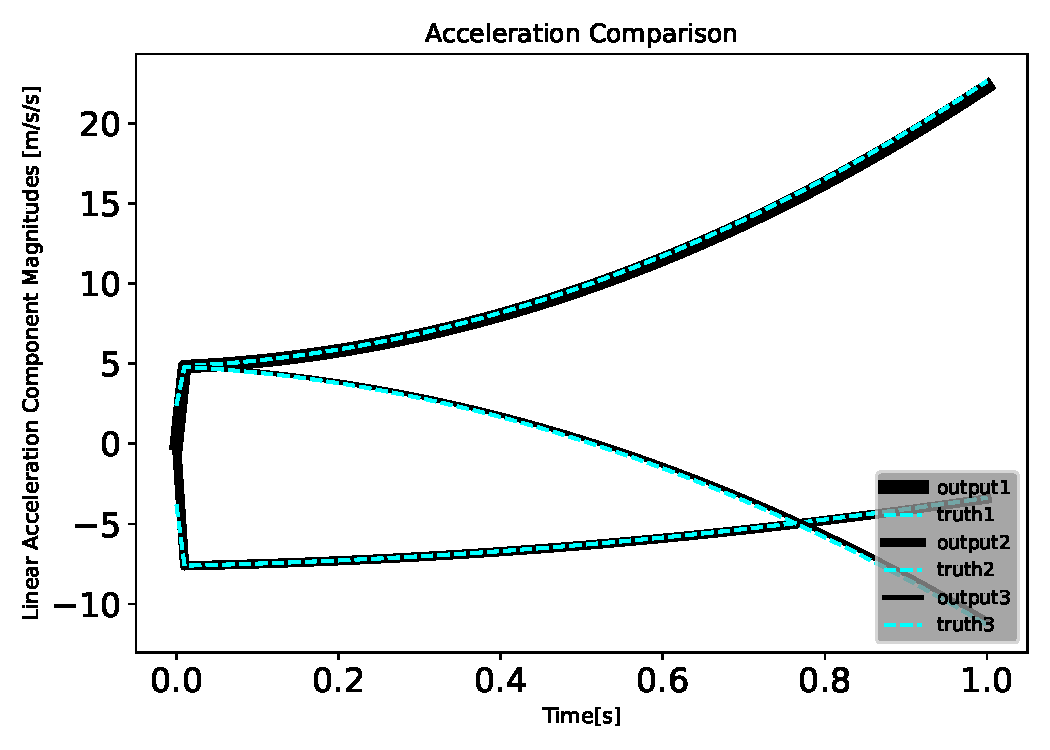
\includegraphics[height=0.7\textwidth, keepaspectratio]{AutoTeX/cleanaccelComparison}}\caption{Plot Comparing Sensor Linear Accelertaion Truth and Output for test: clean. Note that 1, 2, and 3 indicate the components of the acceleration.}\label{fig:cleanaccelComparison}\end{figure}
\begin{figure}[htbp]\centerline{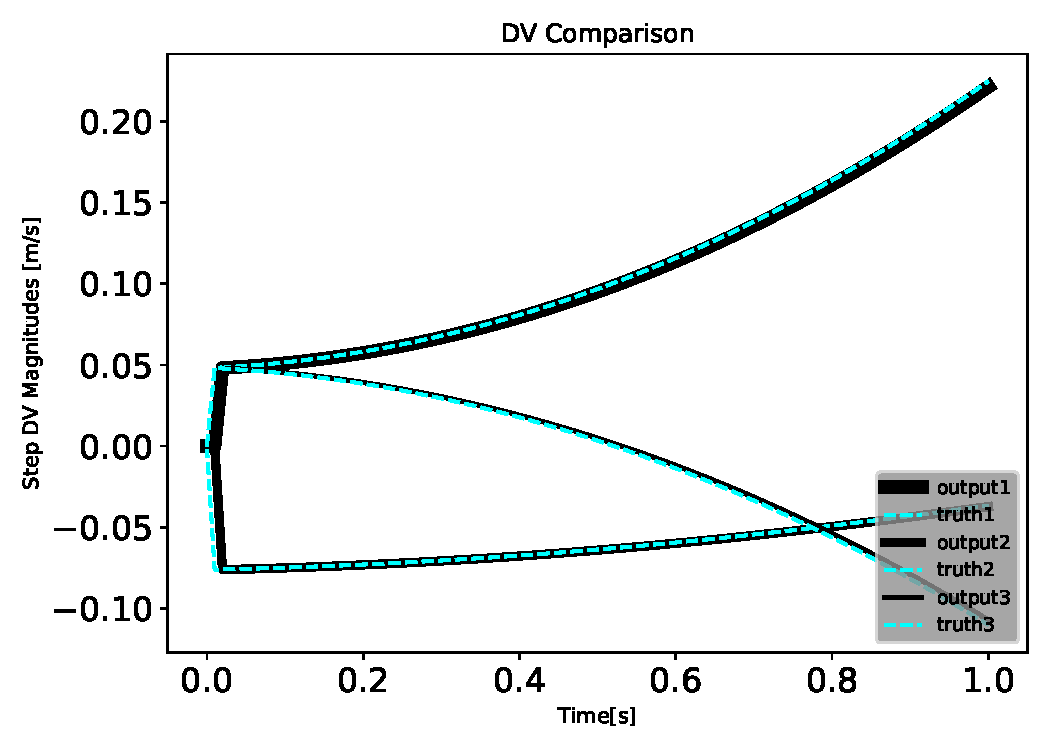
\includegraphics[height=0.7\textwidth, keepaspectratio]{AutoTeX/cleanDVcomparison}}\caption{Plot Comparing Time Step DV Truth and Output for test: clean. Note that 1, 2, and 3 indicate the components of the velocity delta.}\label{fig:cleanDVcomparison}\end{figure}
\begin{figure}[htbp]\centerline{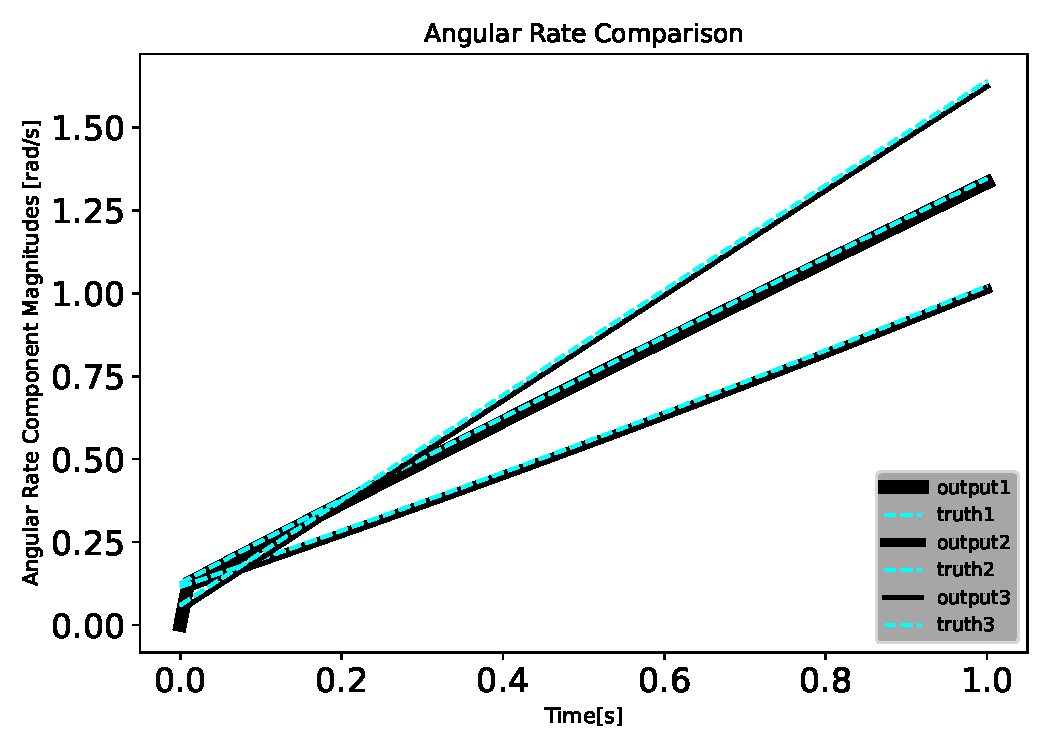
\includegraphics[height=0.7\textwidth, keepaspectratio]{AutoTeX/cleanomegaComparison}}\caption{Plot Comparing Angular Rate Truth and Output for test: clean. Note that 1, 2, and 3 indicate the components of the angular rate.}\label{fig:cleanomegaComparison}\end{figure}
\begin{figure}[htbp]\centerline{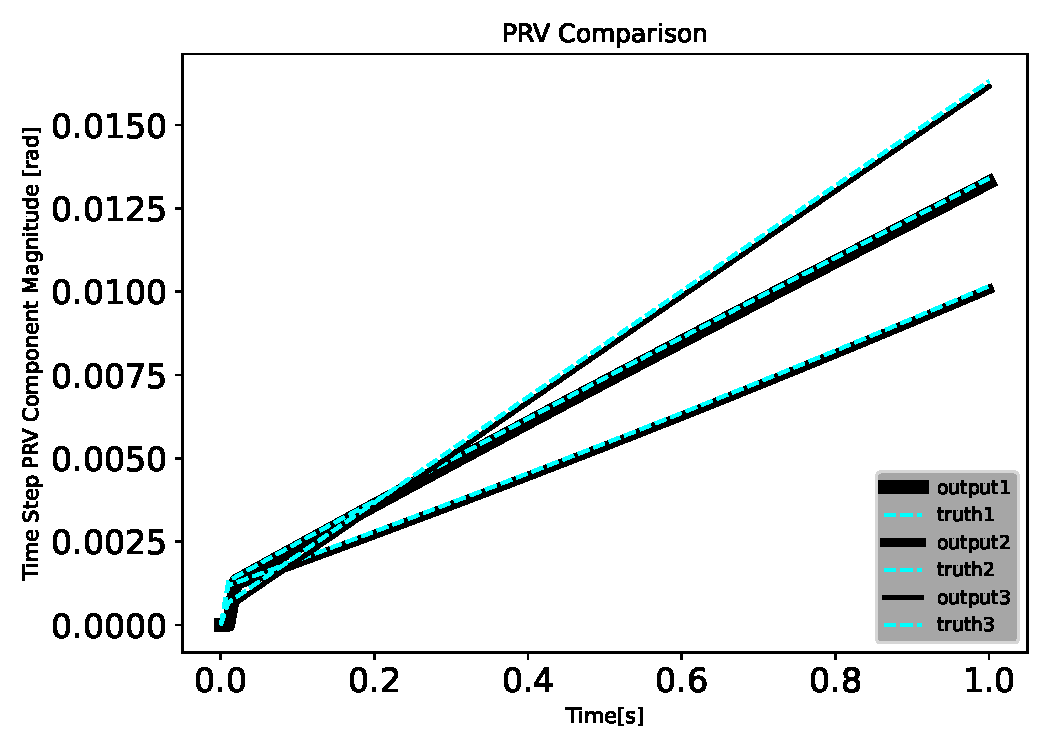
\includegraphics[height=0.7\textwidth, keepaspectratio]{AutoTeX/cleanPRVcomparison}}\caption{Plot Comparing Time Step PRV Truth and Output for test: clean. Note that 1, 2, and 3 indicate the components of the principal rotation vector.}\label{fig:cleanPRVcomparison}\end{figure}

\clearpage

\begin{figure}[htbp]\centerline{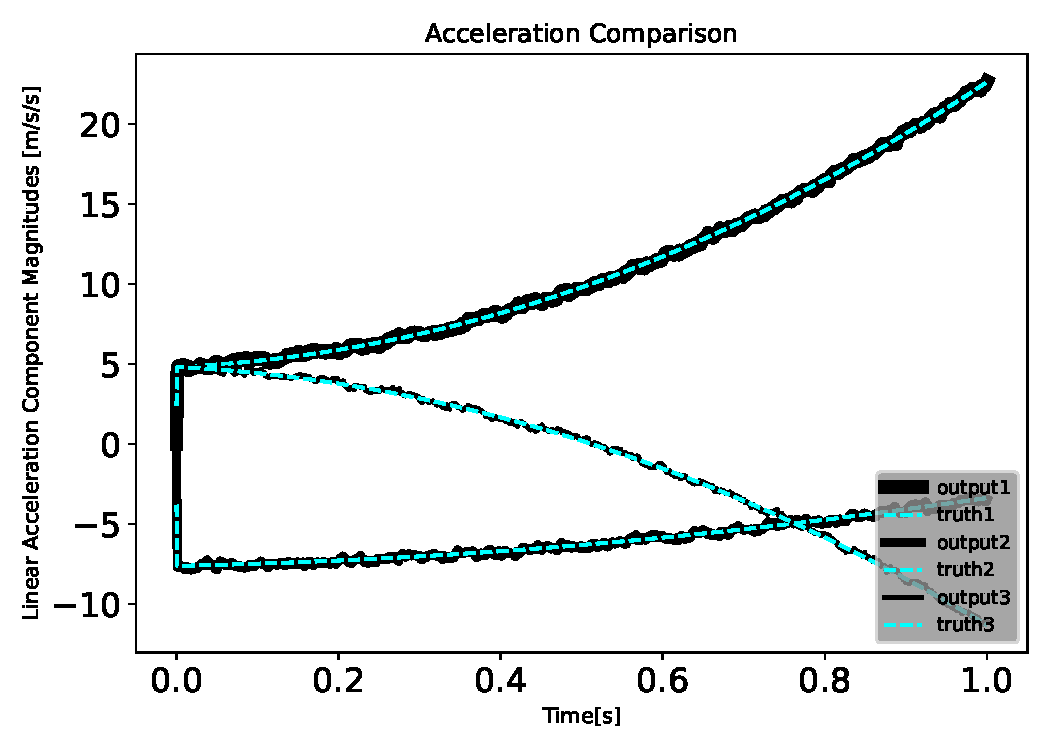
\includegraphics[height=0.7\textwidth, keepaspectratio]{AutoTeX/noiseaccelComparison}}\caption{Plot Comparing Sensor Linear Accelertaion Truth and Output for test: noise. Note that 1, 2, and 3 indicate the components of the acceleration.}\label{fig:noiseaccelComparison}\end{figure}
\begin{figure}[htbp]\centerline{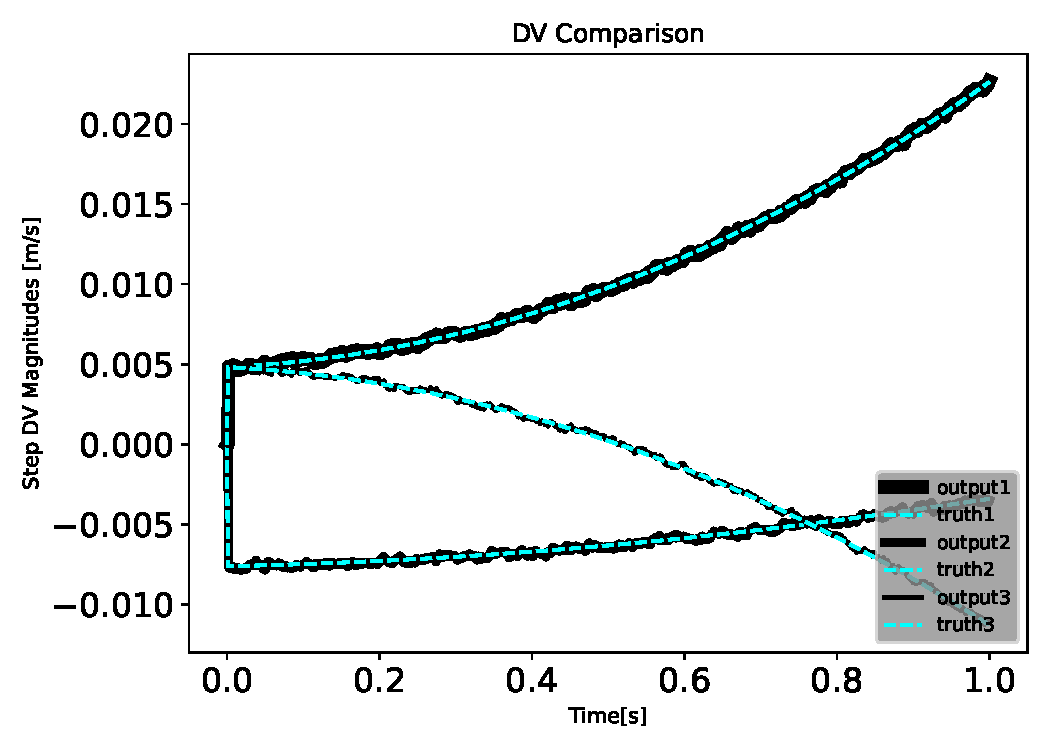
\includegraphics[height=0.7\textwidth, keepaspectratio]{AutoTeX/noiseDVcomparison}}\caption{Plot Comparing Time Step DV Truth and Output for test: noise. Note that 1, 2, and 3 indicate the components of the velocity delta.}\label{fig:noiseDVcomparison}\end{figure}
\begin{figure}[htbp]\centerline{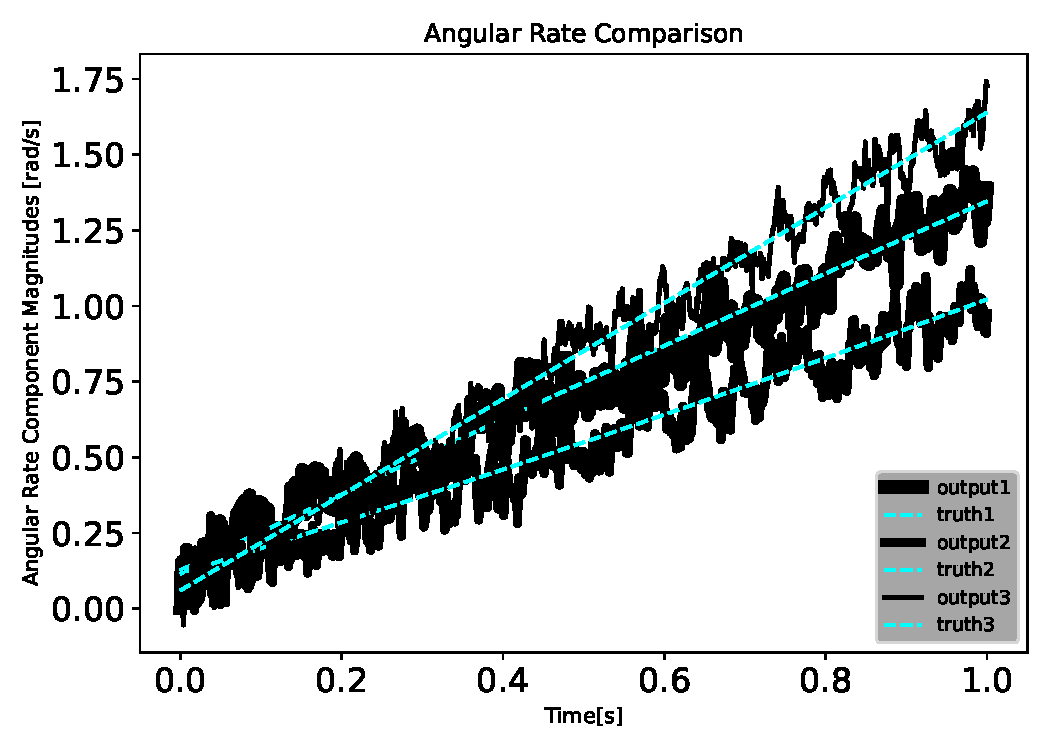
\includegraphics[height=0.7\textwidth, keepaspectratio]{AutoTeX/noiseomegaComparison}}\caption{Plot Comparing Angular Rate Truth and Output for test: noise. Note that 1, 2, and 3 indicate the components of the angular rate.}\label{fig:noiseomegaComparison}\end{figure}
\begin{figure}[htbp]\centerline{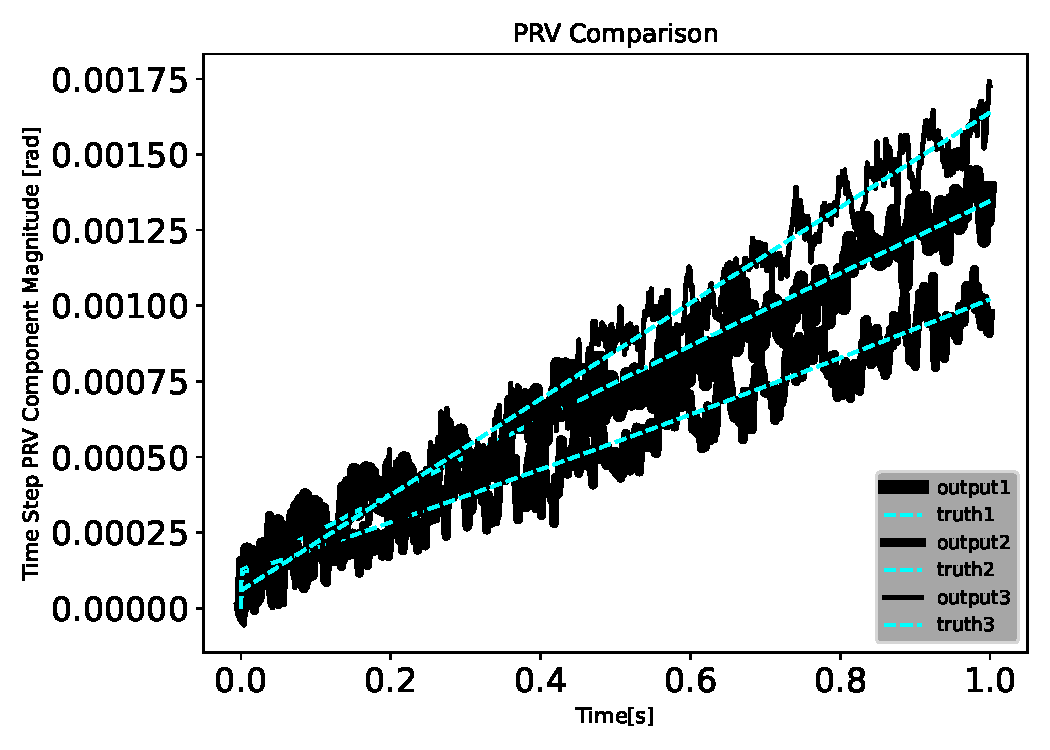
\includegraphics[height=0.7\textwidth, keepaspectratio]{AutoTeX/noisePRVcomparison}}\caption{Plot Comparing Time Step PRV Truth and Output for test: noise. Note that 1, 2, and 3 indicate the components of the principal rotation vector.}\label{fig:noisePRVcomparison}\end{figure}

\clearpage

\begin{figure}[htbp]\centerline{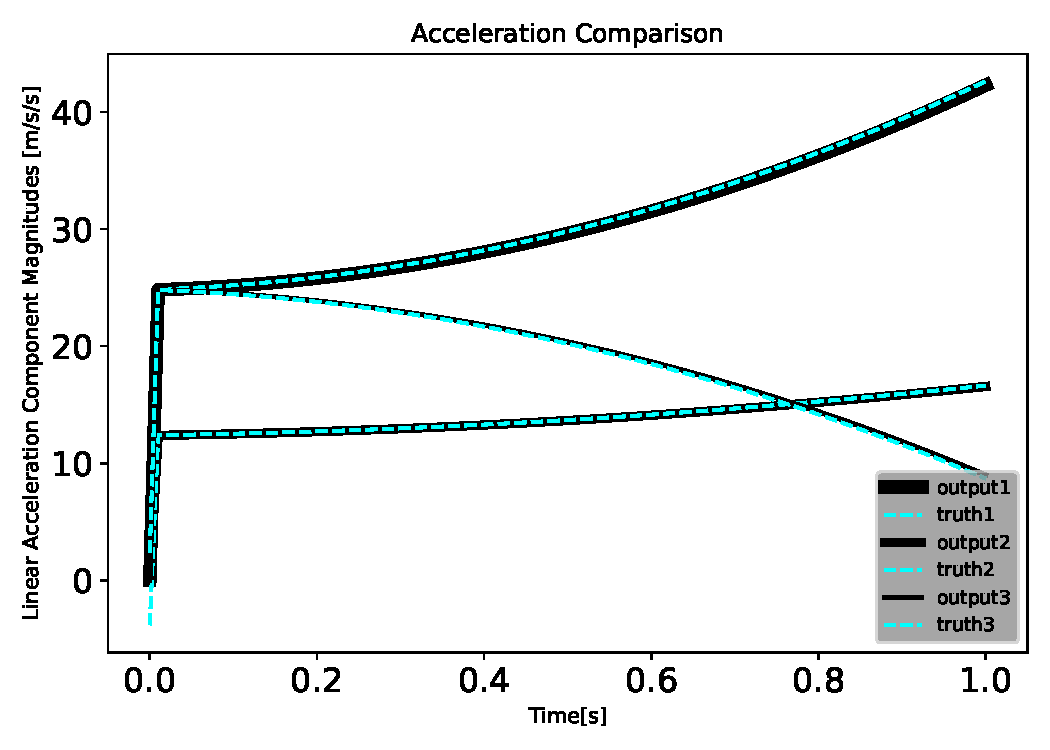
\includegraphics[height=0.7\textwidth, keepaspectratio]{AutoTeX/biasaccelComparison}}\caption{Plot Comparing Sensor Linear Accelertaion Truth and Output for test: bias. Note that 1, 2, and 3 indicate the components of the acceleration.}\label{fig:biasaccelComparison}\end{figure}
\begin{figure}[htbp]\centerline{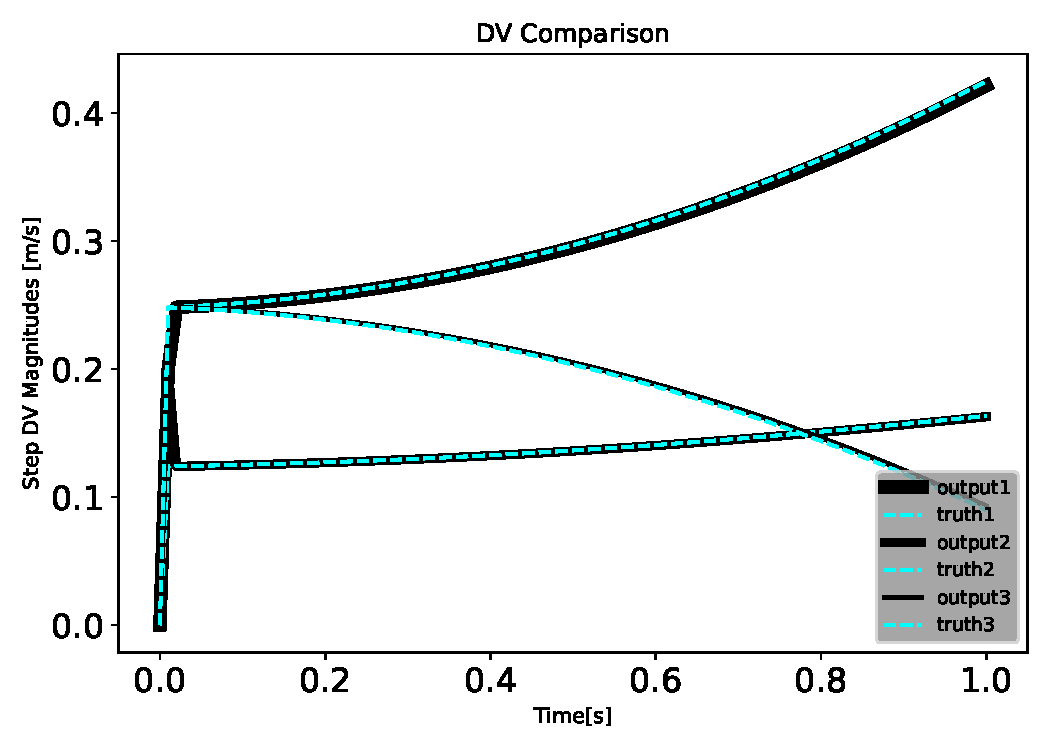
\includegraphics[height=0.7\textwidth, keepaspectratio]{AutoTeX/biasDVcomparison}}\caption{Plot Comparing Time Step DV Truth and Output for test: bias. Note that 1, 2, and 3 indicate the components of the velocity delta.}\label{fig:biasDVcomparison}\end{figure}
\begin{figure}[htbp]\centerline{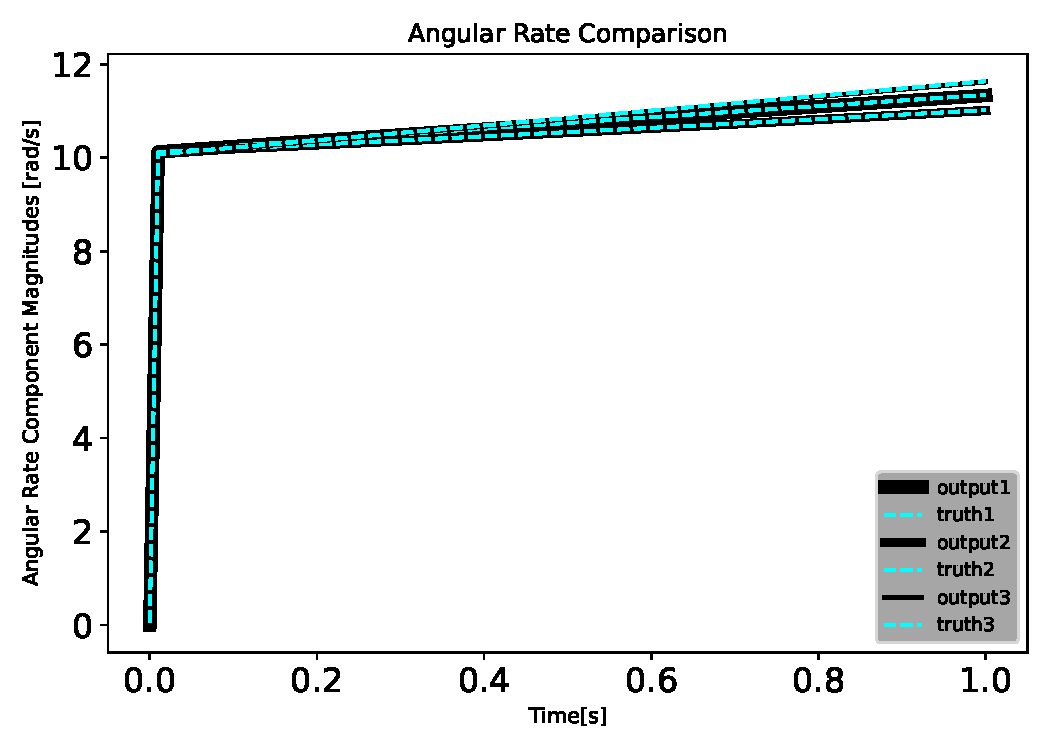
\includegraphics[height=0.7\textwidth, keepaspectratio]{AutoTeX/biasomegaComparison}}\caption{Plot Comparing Angular Rate Truth and Output for test: bias. Note that 1, 2, and 3 indicate the components of the angular rate.}\label{fig:biasomegaComparison}\end{figure}
\begin{figure}[htbp]\centerline{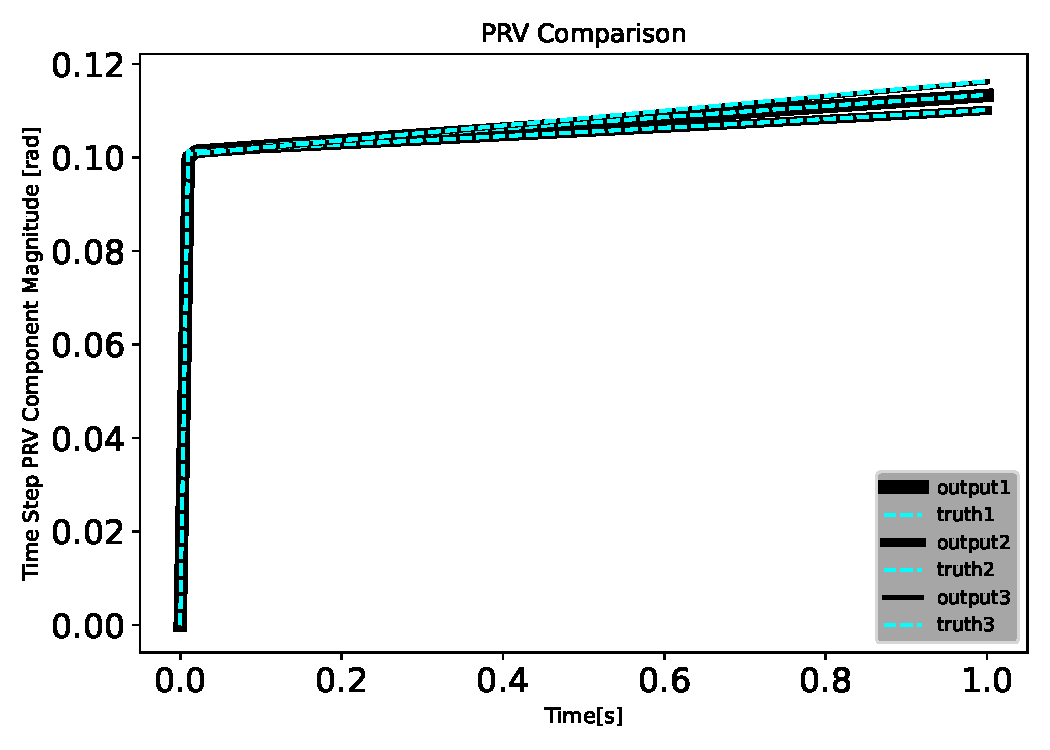
\includegraphics[height=0.7\textwidth, keepaspectratio]{AutoTeX/biasPRVcomparison}}\caption{Plot Comparing Time Step PRV Truth and Output for test: bias. Note that 1, 2, and 3 indicate the components of the principal rotation vector.}\label{fig:biasPRVcomparison}\end{figure}

\clearpage

\begin{figure}[htbp]\centerline{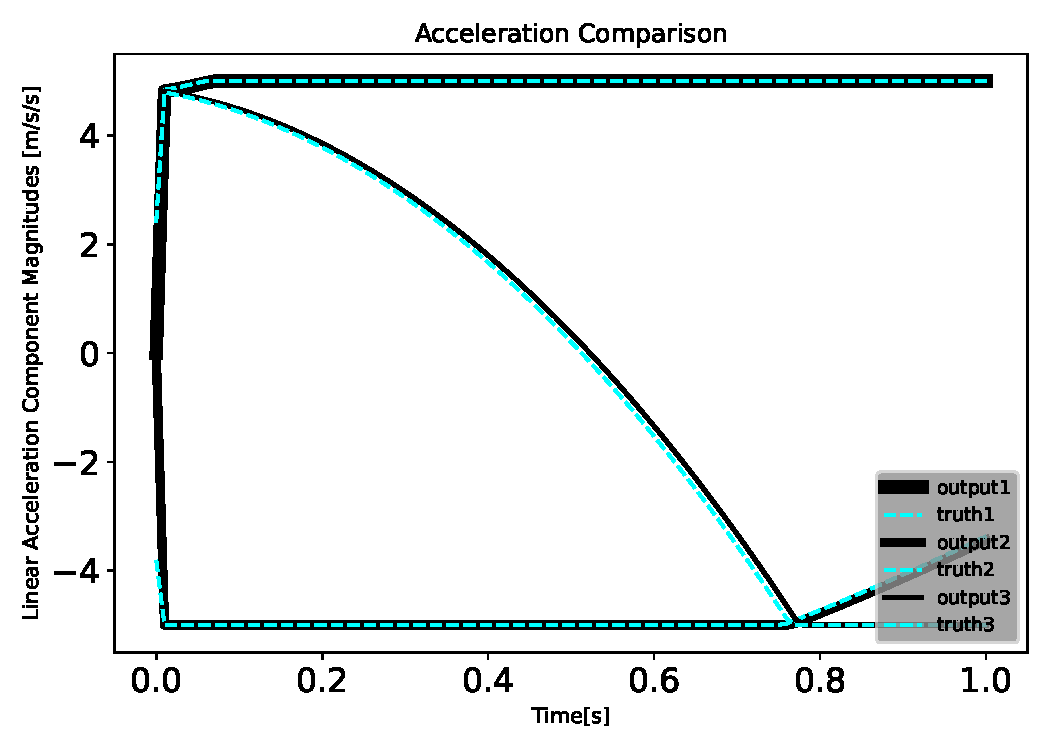
\includegraphics[height=0.7\textwidth, keepaspectratio]{AutoTeX/saturationaccelComparison}}\caption{Plot Comparing Sensor Linear Accelertaion Truth and Output for test: saturation. Note that 1, 2, and 3 indicate the components of the acceleration.}\label{fig:saturationaccelComparison}\end{figure}
\begin{figure}[htbp]\centerline{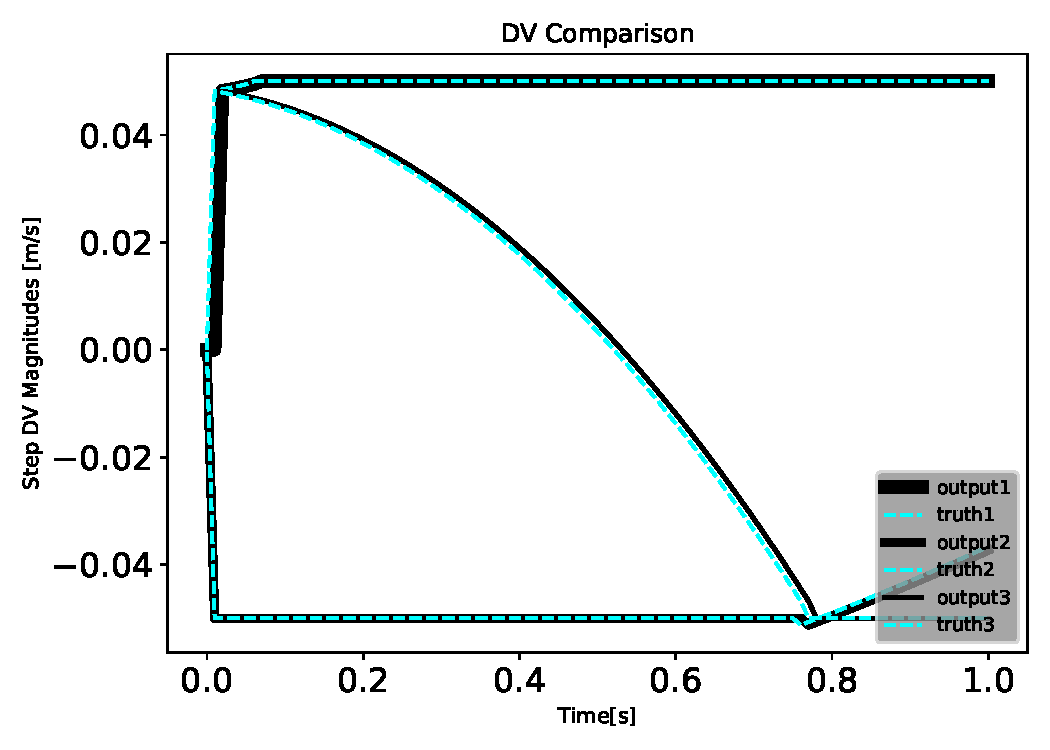
\includegraphics[height=0.7\textwidth, keepaspectratio]{AutoTeX/saturationDVcomparison}}\caption{Plot Comparing Time Step DV Truth and Output for test: saturation. Note that 1, 2, and 3 indicate the components of the velocity delta.}\label{fig:saturationDVcomparison}\end{figure}
\begin{figure}[htbp]\centerline{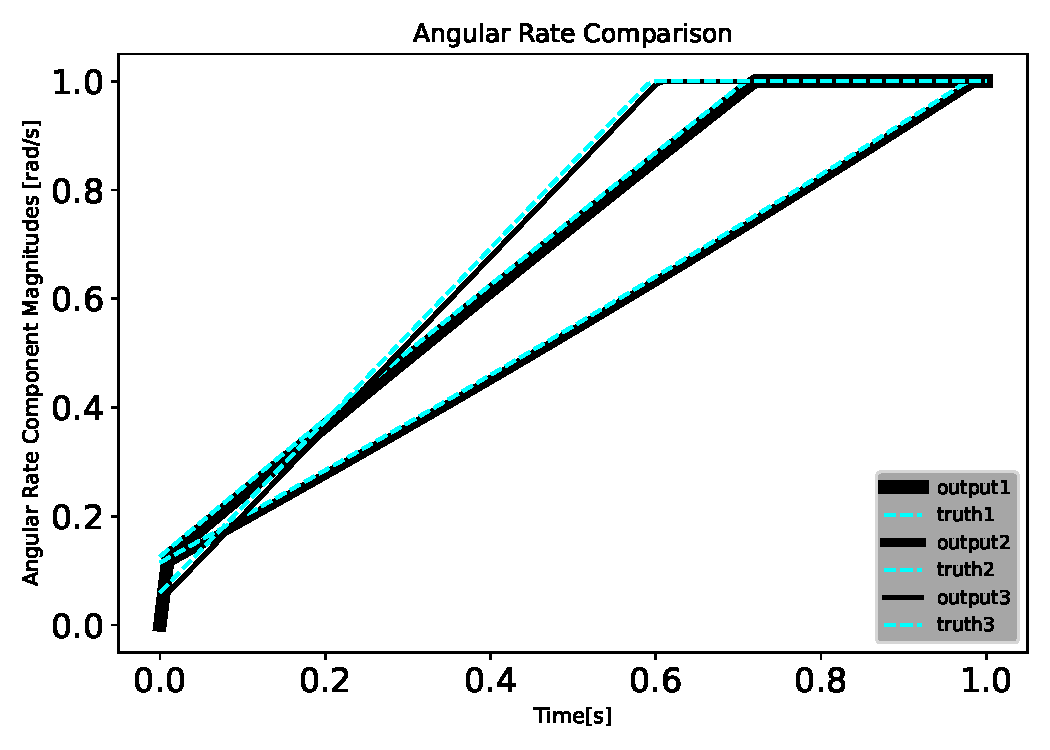
\includegraphics[height=0.7\textwidth, keepaspectratio]{AutoTeX/saturationomegaComparison}}\caption{Plot Comparing Angular Rate Truth and Output for test: saturation. Note that 1, 2, and 3 indicate the components of the angular rate.}\label{fig:saturationomegaComparison}\end{figure}
\begin{figure}[htbp]\centerline{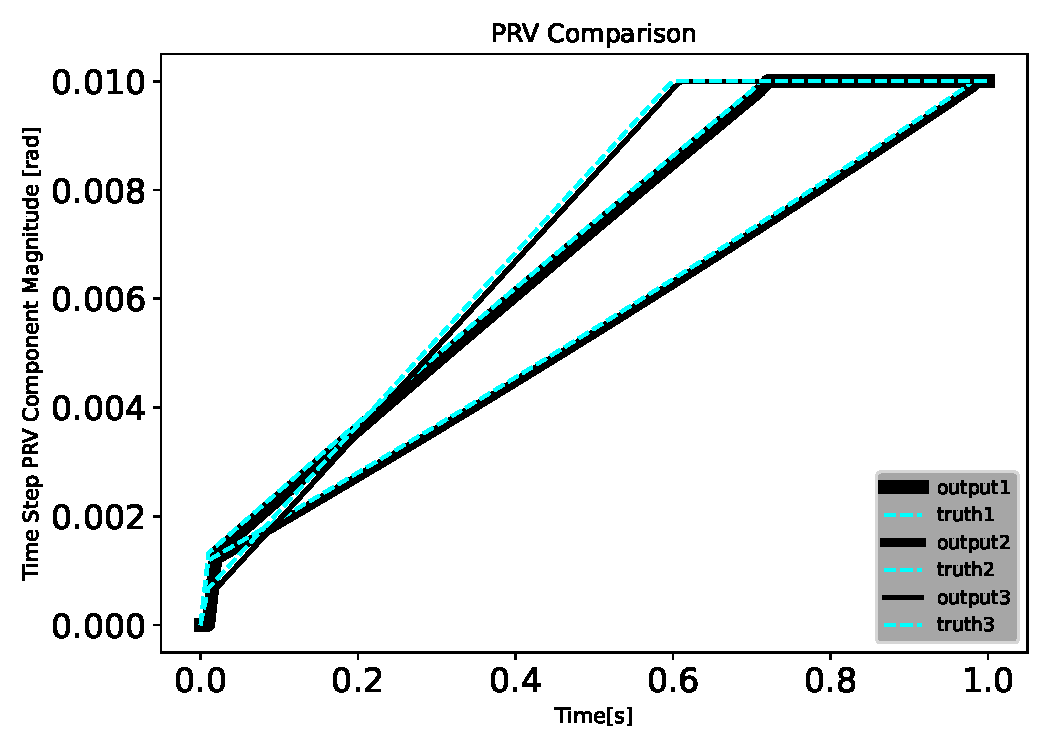
\includegraphics[height=0.7\textwidth, keepaspectratio]{AutoTeX/saturationPRVcomparison}}\caption{Plot Comparing Time Step PRV Truth and Output for test: saturation. Note that 1, 2, and 3 indicate the components of the principal rotation vector.}\label{fig:saturationPRVcomparison}\end{figure}

\clearpage

\begin{figure}[htbp]\centerline{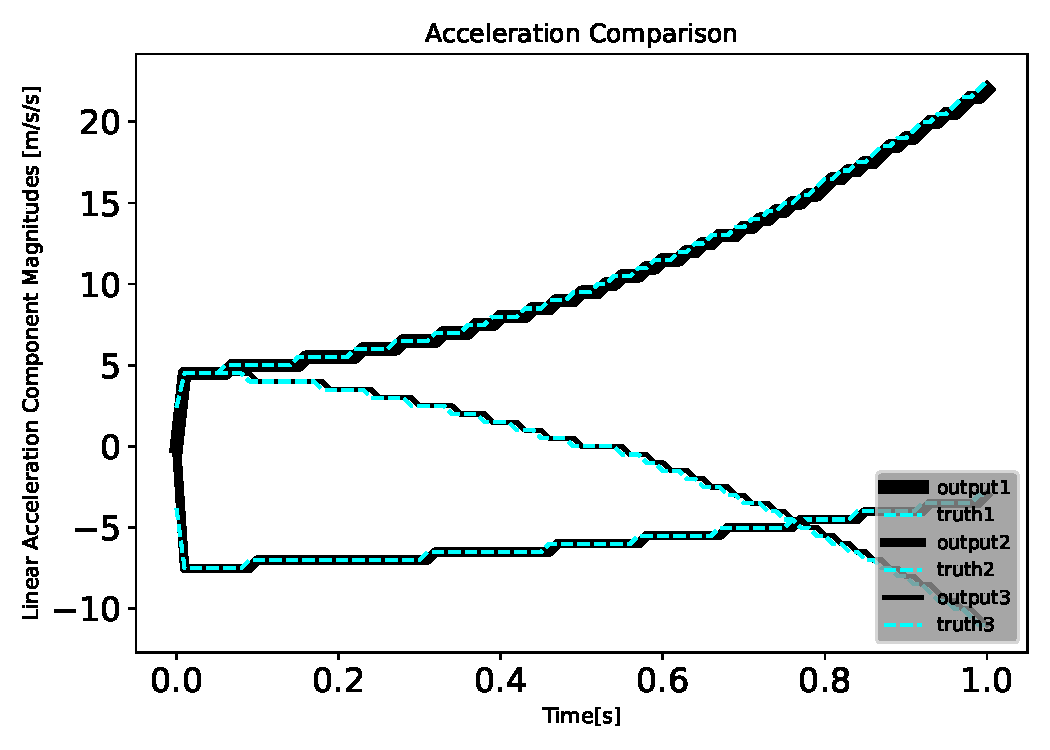
\includegraphics[height=0.7\textwidth, keepaspectratio]{AutoTeX/discretizationaccelComparison}}\caption{Plot Comparing Sensor Linear Accelertaion Truth and Output for test: discretization. Note that 1, 2, and 3 indicate the components of the acceleration.}\label{fig:discretizationaccelComparison}\end{figure}
\begin{figure}[htbp]\centerline{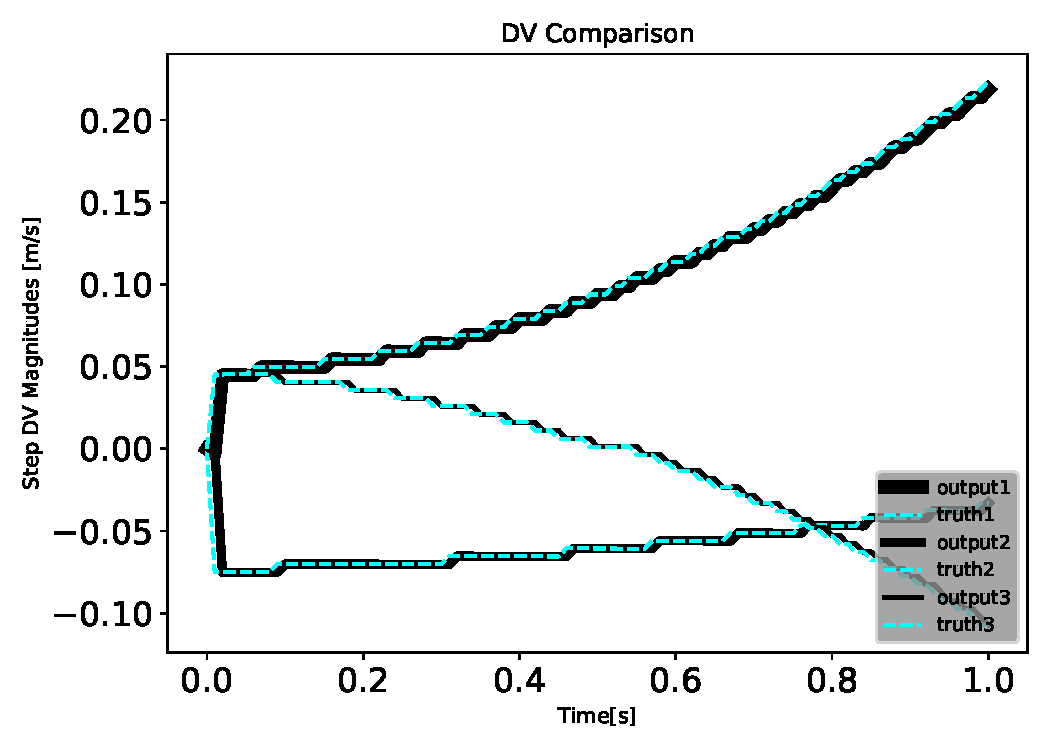
\includegraphics[height=0.7\textwidth, keepaspectratio]{AutoTeX/discretizationDVcomparison}}\caption{Plot Comparing Time Step DV Truth and Output for test: discretization. Note that 1, 2, and 3 indicate the components of the velocity delta.}\label{fig:discretizationDVcomparison}\end{figure}
\begin{figure}[htbp]\centerline{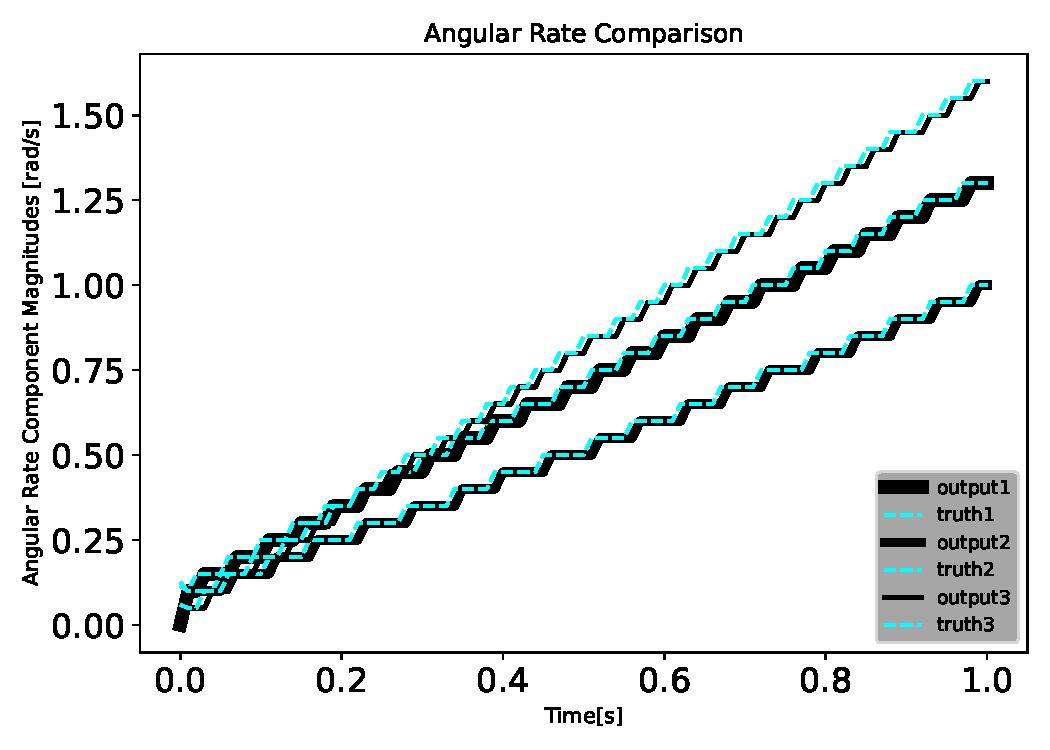
\includegraphics[height=0.7\textwidth, keepaspectratio]{AutoTeX/discretizationomegaComparison}}\caption{Plot Comparing Angular Rate Truth and Output for test: discretization. Note that 1, 2, and 3 indicate the components of the angular rate.}\label{fig:discretizationomegaComparison}\end{figure}
\begin{figure}[htbp]\centerline{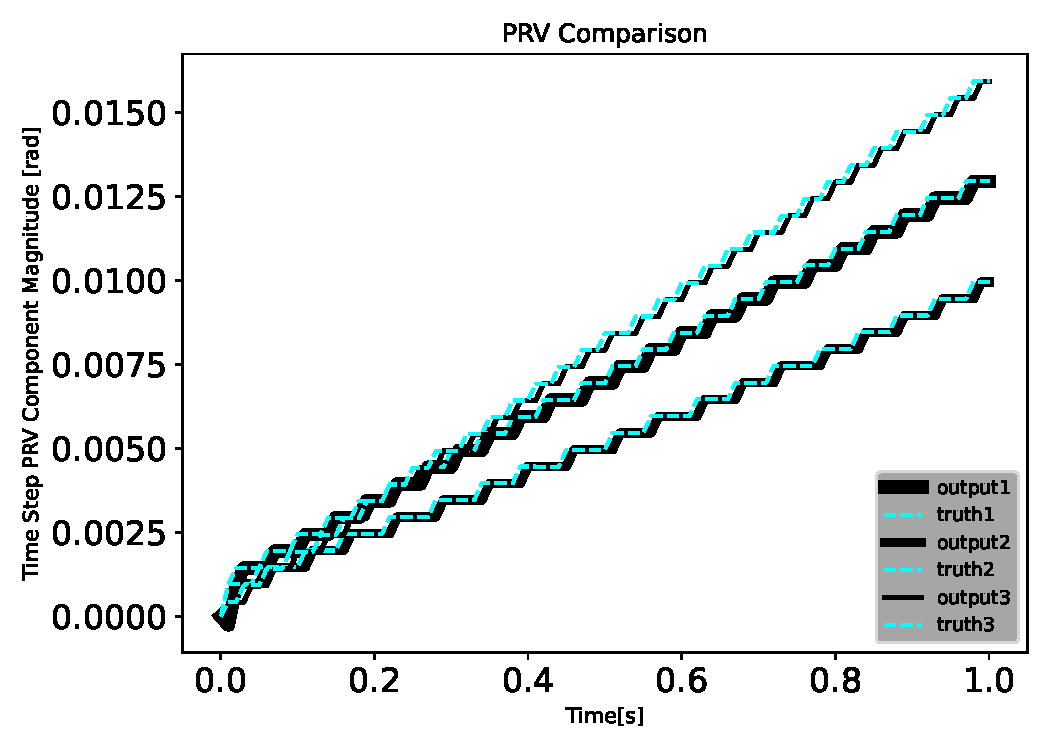
\includegraphics[height=0.7\textwidth, keepaspectratio]{AutoTeX/discretizationPRVcomparison}}\caption{Plot Comparing Time Step PRV Truth and Output for test: discretization. Note that 1, 2, and 3 indicate the components of the principal rotation vector.}\label{fig:discretizationPRVcomparison}\end{figure}

\clearpage

\begin{figure}[htbp]\centerline{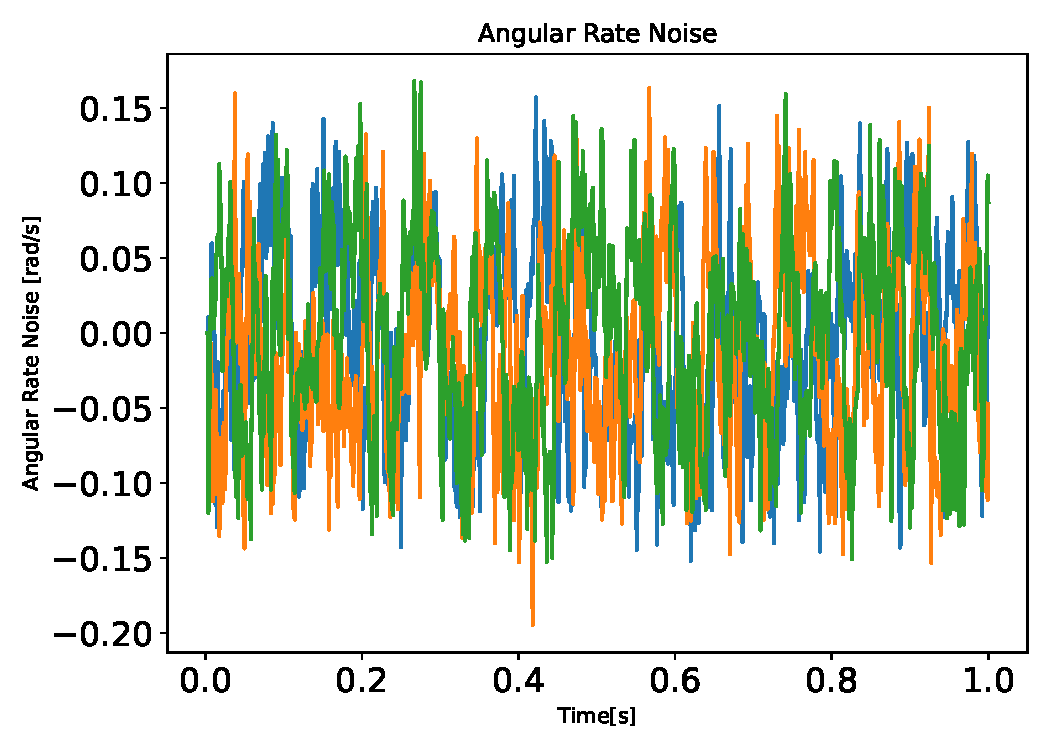
\includegraphics[height=0.7\textwidth, keepaspectratio]{AutoTeX/omegaNoise}}\caption{Plot of Angular Rate noise along each component for the noise test.}\label{fig:omegaNoise}\end{figure}
\begin{figure}[htbp]\centerline{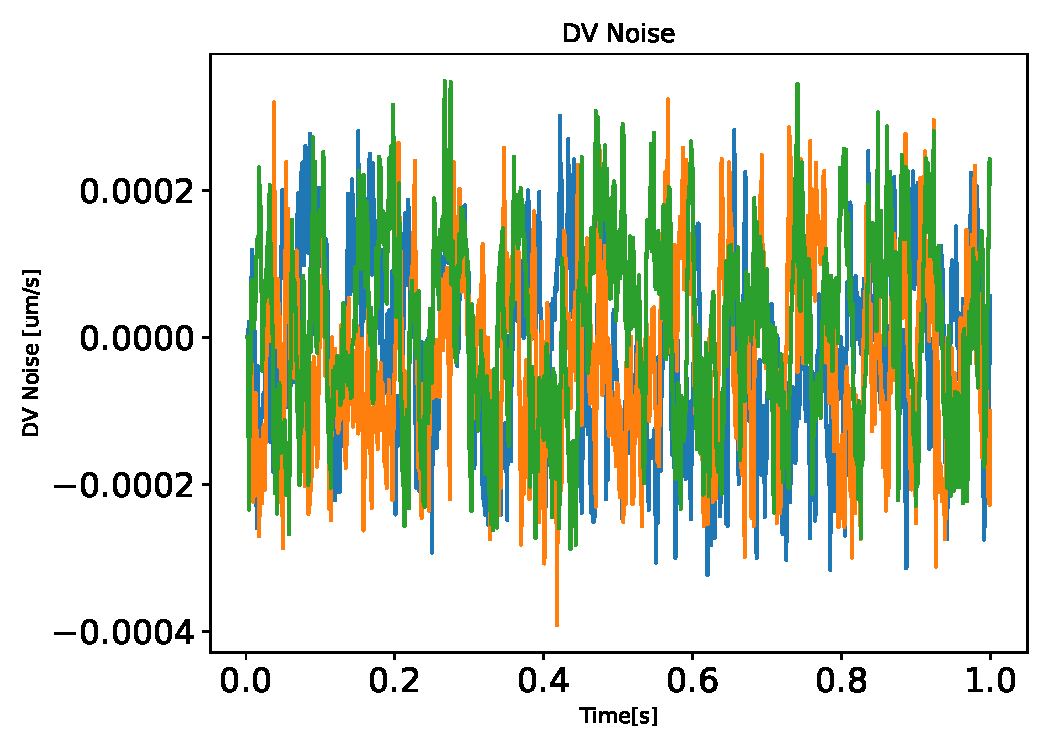
\includegraphics[height=0.7\textwidth, keepaspectratio]{AutoTeX/DVnoise}}\caption{Plot of DeltaV noise along each component for the noise test.}\label{fig:DVnoise}\end{figure}
\begin{figure}[htbp]\centerline{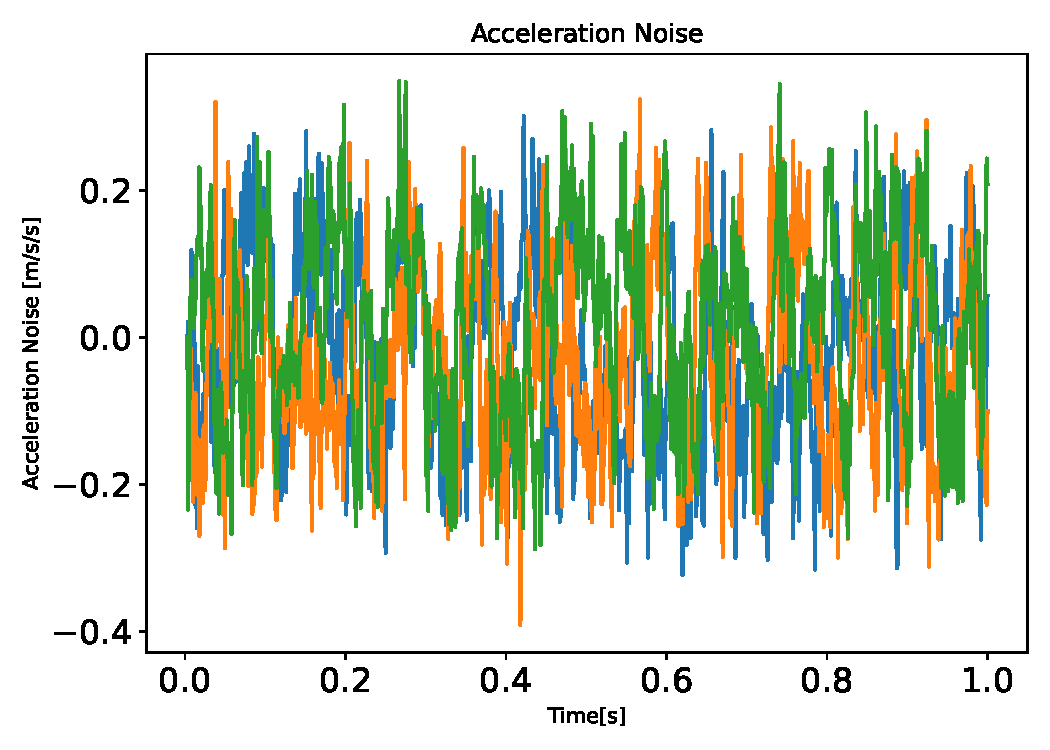
\includegraphics[height=0.7\textwidth, keepaspectratio]{AutoTeX/AccelNoise}}\caption{Plot of acceleration noise along each component for the noise test.}\label{fig:AccelNoise}\end{figure}
\begin{figure}[htbp]\centerline{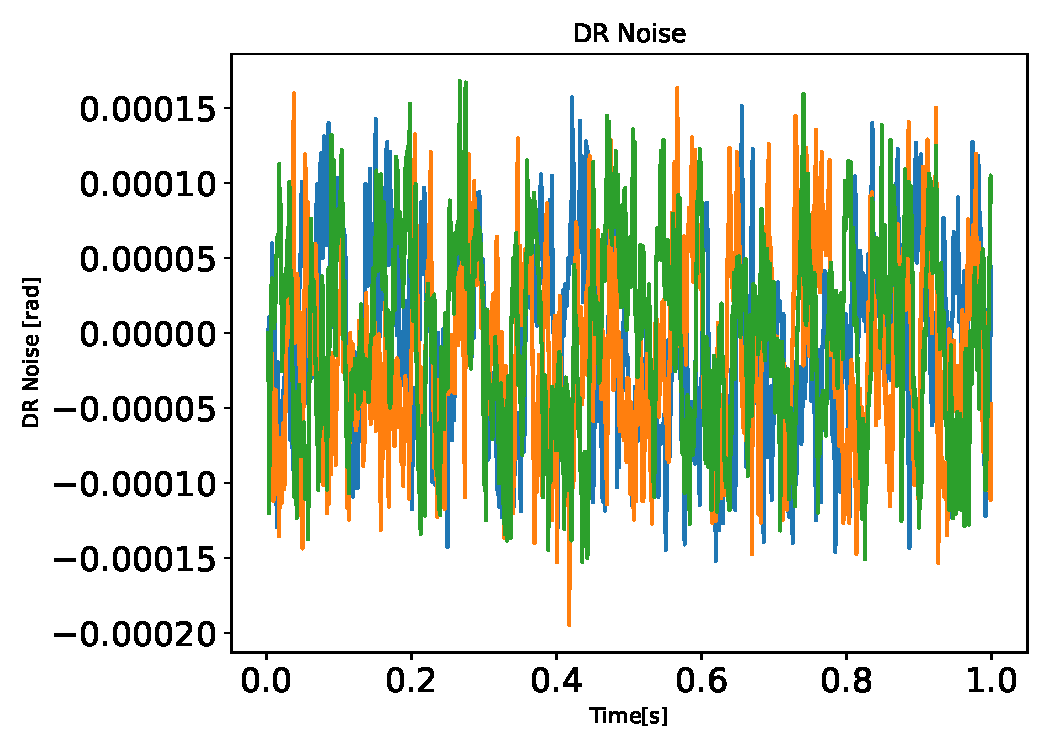
\includegraphics[height=0.7\textwidth, keepaspectratio]{AutoTeX/DRnoise}}\caption{Plot of PRV noise along each component for the noise test.}\label{fig:DRnoise}\end{figure}

\pagebreak %needed to keep images/paragraphs in the right place. Cannot \usepackage{float} here because it is not used in the AutoTex implementation.